\chapter{Software and Computing}
\label{ch:detectors-sc}

\section{Computing Infrastructure}
\label{sec:detectors-sc-infrastructure}

\subsection{Raw Data Rates}
\label{sec:detectors-sc-infrastructure-data-rates}
\fixme{A special Annex document for data rates was updated on 4/13/2015. It covers most DUNE physics and background
processes but the information is incomplete. Currently this S\&C section is being updated to include references to the Annex.}



\subsubsection{Raw Data Streams}
DUNE is a multipurpose apparatus and the variety of physics goals to be pursued during its operation will
be reflected in different characteristics of respective data streams processed and collected in real time and off-line.
As one example, consider the difference between neutrino oscillations physics done with beam neutrinos on one hand,
and the ambitious goal of detecting the rare Supernova bursts (SNB) on the other. Signals produced by ``beam events'' will
be characterzied by energies in the GeV range, allowing appropriate thresholds for zero-suppression (ZS) to be
set at the levels which greatly reduce the background component of the data. By comparison, the energy scale of
the signals produced by SNB neutrino interactions in the active volume of the detector is estimated to be in the range of tens of MeV, resulting
in much lower thresholds to be set for this type of measurement, and therefore in considerable (if not overwhelming) volume of SNB-specific data coming
out of the LAr TPC in real time and being dominated by radiological backgrounds. Another differentiating SNB feature is that multiple neutrinos are expected
to arrive and interact in the detector during the possible rare Supernova burst event within seconds from each other, as opposed to a rare single vertex produced by a beam neutrino.
To support SNB physics, a massive burst of noisy data will need to be processed ``on the fly'' using approaches and
algorithms which are completely  different from those for the beam neutrino physics, which mostly relies on off-line processing.

Distinctions such as this one are made here in order to define the scope of this section, which focuses on data streams present in
oscillation physics studies, since these data will constitute the bulk of what's committed to mass storage, transmitted over networks,
processed offline and in general have significant infrastructure and cost implications. Issues and parameters related to other classes of data are covered in
the Annex to this document, titled ``Characterization of Data Rates and Volumes for specific sources of activity in DUNE Detectors'',
and also in the DAQ and other sections.

\subsubsection{Assumptions}
\label{sec:detectors-sc-infrastructure-assumptions}
According to the present baseline design, the Far Detector (Liquid Argon TPC) in DUNE will consist of four identical modules of 10kt each.
For purposes of this document the issue of possible variations in the design and/or characteristics between
these modules shall not be addressed, as there is no concrete information developed at this point to support this approach. A few basic assumptions
will need to be used:
\begin{itemize}
\item Estimates presented below correspond to the ``full detector'', i.e. is effectively normalized to 40kt.
\item Accelerator spill cycle is 1.2s
\item Zero-Suppression thresholds will be set at levels corresponding to self-triggered data being read out every spill cycle.
\item The intensity of the beam provided by LBNF will affect the data rates for a few detector systems in DUNE (cf. the Near Detector).
It is assumed that the beam has the characteristics suggested by LBNF Project at the time of writing.
\item It is assumed that the front-end systems of the TPC and the Photon Detector combined with the logic in DAQ
will provide triggering capability for the beam neutrino physics.
\end{itemize}
\
Certain parameters may be rounded off where appropriate.

\subsubsection{DUNE Detector Subsystems}
\begin{itemize}
\item Far Detector LAr TPC, Photon Detector(PD)
\item Near Detector (ND) Straw Tracker (STT), Calorimeter(CAL), Muon Detector Resistive Plate Chambers (RPC)
\end{itemize}

In the following, estimated data rates for these components are itemized and then aggregated.
There will be cases where no reliable estimates exist at the moment due to continued R\&D, and this will be clearly stated where necessary.

\subsubsection{Far Detector LAr TPC}
Relevant  LAr TPC parameters:
\begin{itemize}
\item Readout channel count: 1,536,000 (i.e. four times 384,000 which is the channel count for each 10kt module)
\item Drift Time: approx. 2ms
\item ADC clock frequency: approx. 2MHz
\item ADC resolution (bits): 12
\end{itemize}
\
Factors affecting data rates:
\begin{itemize}
\item Zero Suppression (ZS)  in the Front-End electronics of the detector
\item Radiological and Cosmological Backgrounds as functions of thresholds set for ZS, in different physics domains (cf. beam neutino physics vs Supernova Burst)
\end{itemize}

Non-ZS maximum event size (corresponding to a snapshot of the complete TPC) can be calculated as a product of the following numbers:
\begin{itemize}
\item Channel count
\item Number of ADC ``clicks'' per total drift (collection) time
\item ADC resolution
\end{itemize}
\
This results in a total of 9.2GB worth of TPC data. According to current estimates, with thresholds optimized for beam neutrino physics, zero suppression
gives us a reduction factor of \textasciitilde 100 in the event size, resulting in a 92~MB ``digital picture'' of the beam neutrino event in the TPC
(discriminated against most background but \textit{still covering the complete volume of the TPC}).
Since neutrino interactions will result in a more local pattern of ionization signal being read out
from the chamber, Monte Carlo studies done with realistic neutrino energy spectra suggest between 10 and 20MB per neutral current event.
Following the threshold levels assumption in ~\ref{sec:detectors-sc-infrastructure-assumptions}, one arrives at the number of \textasciitilde 20MB/s for the data rate
which only includes the beam neutrino type of events. This translates into \textasciitilde 0.6PB/year.

%As discussed above, most of implications of the SNB signal and trigger are mostly relevant for the front-end and DAQ system, however it's worthwhile to
%understand what needs to be provided to preserve such possible signal and commit data to mass storage. There are many uncertainties about signatures
%and signal to noise ratio for the relevant reactions in the detector volume, but it's safe to assume that the thresholds for such events will need to be set
%at very low levels and the data will be dominated by radiological backgrounds.


\subsubsection{Far Detector Photon Detector (PD)}
Relevant  PD parameters:
\begin{itemize}
\item Readout channel count: 24,000 (i.e. four times 6,000 which is the channel count for each 10kt module)
\item Trigger rate is uncertain at this point due to ongoing investigation; one approach that exists assumes 1 trigger per spill cycle
\item ADC resolution (bits): 12
\end{itemize}
\
This results in 36kB per spill cycle, and should be considered negligible from the point of view of requirement to data handling, compared to other data sources.

\subsubsection{Near Detector Data Rates}
Relevant parameters of the Fine-Grained Tracker (FGT):
\begin{itemize}
\item   Straw Tube Tracker (STT) readout channel count: 215,040
\item STT Drift Time: 120ns
\item STT ADC clock frequency and resolution (bits): 3ns intervals, 10 bit
\item ECAL channel count: 52,224
\item Muon Detector Resistive Plane Chambers (RPC) channel count: 165,888
\item Average expected event rate per spill: \textasciitilde 1.5
\end{itemize}
\
Based on these parameters, the upper limit of the ND data rate can be estimated as 1.5MB/s. This translates into \textasciitilde 45TB/year. 

\subsection{Processed Data}
\label{sec:detectors-sc-infrastructure-processed-data}
For the purposes of this document, processed data is defined as most data which is not considered ``raw'', i.e. it's data derived from raw (including possibly multiple stages
of calibration and reconstruction) as well as data produced as a result of Monte Carlo studies.

There are uncertainties in anticipated quantities of all of these types of data, but based on the estimated annual raw data volume of 0.6PB, and assuming that
the data will undergo a few processing stages, one can expect the need to handle \textasciitilde 2PB of data annually for reconstruction and a lesser
volume for final analysis purposes.

For Monte Carlo, at the time of writing typical annual volume of data produced has been of the order of a few tens of terabytes. With Collaboration growing
and more detailed studies (e.g. of systematics) are undertaken, our expectation is that DUNE will require 100TB annually for storage of its MC data.

\subsection{Computing Model}
\label{sec:detectors-sc-infrastructure-computing-model}

\subsubsection{Distributed Computing}

Given the fact the Collaboration is large and widely dispersed geographically, a fully distributed approach to computing is recommended, based on experience
gained during the operation of the LHC experiments. This will allow the DUNE Collaboration to better leverage resources and expertise from many of its
member institutions and improve the overall long-term scalability of its computing platform.

DUNE will operate a  distributed network of federated resources, for both CPU power and storage capability. This will allow for streamlined incorporation
of computing facilities as they become available at member institutions, and thus is particularly amenable to accommodate staged construction and commissioning
of the detector subsystems. A modern Workload Management System will be deployed on top of Grid and Cloud resources to provide computing
power to DUNE researchers.

\subsubsection{Raw Data Transmission and Storage Strategy}
FNAL will be the principal data storage center for the experiment. It will serve as a hub where the data from both the Facility (e.g. beam and target)
and the various detector systems (such as the  Far and Near Detectors)  are collected, catalogued and committed to mass storage. This will obviously require transmission of
data over considerable distances (certainly for the Far Detector). In addition, the DAQ systems of the Far Detector are being designed to be located  in the vicinity of
the Far Detector (in the cavern), which results in an additional step of transmitting the data from 4850L to the surface.

Raw data to be collected from the detectors in DUNE are considered ``precious'' due to high cost of operating the both the facility at FNAL
and the detectors that are part of DUNE. This leads to three basic design elements in the data transmission and storage chain:
\begin{itemize}
\item Buffering:
\begin{itemize}
\item Adequate buffers will be provided for the DAQ systems  to mitigate possible downtime of the network connection between 4850L and the surface.
\item Buffers will be provided at the surface facility to mitigate downtime of the network connection between the Far Site and FNAL.
\end{itemize}
\item Robust transmission: data transfer needs to be instrumented with redundant checks (such as checksum calculation), monitoring, error correction and retry logic.
\item Redundant replicas: it is a common industry practice to have a total of three copies of ``precious'' data, which are geographically distributed. This provides protection against catastrophic events (such as natural disasters) at any given data center participating in this scheme, and facilitates rebuilding (``healing'')  lost data should such event does happen.
\end{itemize}



\subsubsection{Data Management}
\label{sec:detectors-sc-infrastructure-computing-model-data-mgt}

Data will be placed into mass storage at FNAL. Along the lines described above, additional copies (replicas) will be distributed to other
computing centers possessing sufficient resources.
A single additional copy does not necessarily need to reside in its entirety on a single data center; the replicas can be ``striped'' across a few data centers if that
becomes optimal at the time of implementation of the Computing Model. For example, consideration is given to both Brookhaven National Laboratory
and NERSC as candidates for the placement of extra replicas.

For data distribution, a combination of managed data movement between sites (such as ``dataset subscription'',
primarily for managed production), and a network of XRootD servers to cache processed data and for analysis will be used.
A file catalog and a Meta-Data system will be required for efficient data management at scale, and an effort will be made to leverage experience of
member institutions in this area, making an effort to reuse existing systems or design ideas where possible.


\section{Far Detector Physics Software}
\label{sec:detectors-sc-physics-software}

%\subsection{Simulation}
%\label{sec:detectors-sc-physics-software-simulation}
% Beam simulation in the Beam Requirements chapter
%\subsubsection{Beam Simulation}
%\label{sec:detectors-sc-physics-software-simulation-beam}
% ND simulation to be dealt with in the ND chapter
%\subsubsection{Near Detector Simulation}
%\label{sec:detectors-sc-physics-software-simulation-nd}

\subsection{Far Detector Simulation}
\label{sec:detectors-sc-physics-software-simulation-fd}

Detailed GEANT4-based~\cite{GEANT4:NIM,GEANT4} Monte Carlo simulations have been 
developed for the single-phase and dual-phase Far Detector designs,
incorporating both the Liquid Argon TPC modules
and the photon detection systems. The simulated data provide
a basis for detailed studies of detector design and performance, 
and enable the development of automated event reconstruction algorithms.

The single-phase detector simulation is implemented in LArSoft~\cite{Church:2013hea},
which provides a common simulation framework for Liquid Argon TPC experiments.
LArSoft is based on the {\it art} framework~\cite{Green:2012gv}, and is supported by Fermilab's
Scientific Computing Division.
The comparison of data from ArgoNeuT~\cite{Anderson:2012vc} with LArSoft
simulations gives confidence in the reliability of the detector simulation.
Future data from LArIAT~\cite{Adamson:2013/02/28tla,Cavanna:2014iqa},
MicroBooNE~\cite{Chen:2007ae,Jones:2011ci,microboonecdr}, and the 35-ton prototype will allow
further tuning of the LArSoft simulation as experience is gained.
The dual-phase detector simulation is based on the Qscan package,
which has been developed over the past decade, and is currently
being used to perform technical design and physics studies for
the \cerndualproto{} program.

Section~\ref{annex:detectors-sc-physics-software-simulation} gives detailed
descriptions of both the single-phase and dual-phase detector simulations.
Events are generated using either the GENIE~\cite{GENIE} simulation of 
neutrino-nucleus interactions, the CRY~\cite{cry} cosmic-ray generator, 
a radiological decay simulator, a particle gun, or one of several
text-file-based particle input sources. GEANT4 is then used to simulate the trajectories
of particles and to model their energy deposition.  
Custom algorithms have been developed to propagate the drifting charge
and scintillation photons through the detector, and to simulate the
response characteristics of the TPC wires, readout electronics, and photon detectors.
Figure~\ref{fig:larsofteventdisplays} shows some examples of accelerator
neutrino interactions simulated using the MicroBooNE detector geometry.

\begin{cdrfigure}[Simulated neutrino interactions in MicroBooNE]{larsofteventdisplays}
{Examples of accelerator neutrino interactions, simulated by LArSoft in the 
MicroBooNE detector. The panels show 2D projections of different event types.
The top panel shows a $\nu_{\mu}$ charged-current interaction with a stopped muon followed
by a decay Michel electron; the middle panel shows a $\nu_{e}$ charged-current 
quasi-elastic interaction with a single electon and proton in the final state;
the bottom panel shows a neutral-current interaction with a $\pi^{0}$ in the final state
that decayed into two photons with separate conversion vertices.}
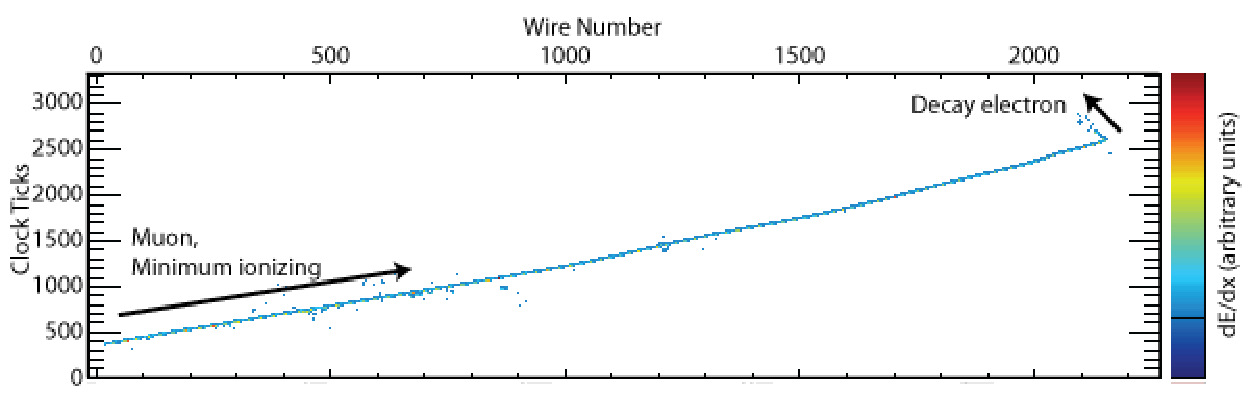
\includegraphics[width=\textwidth]{numuCC_annotated.pdf}
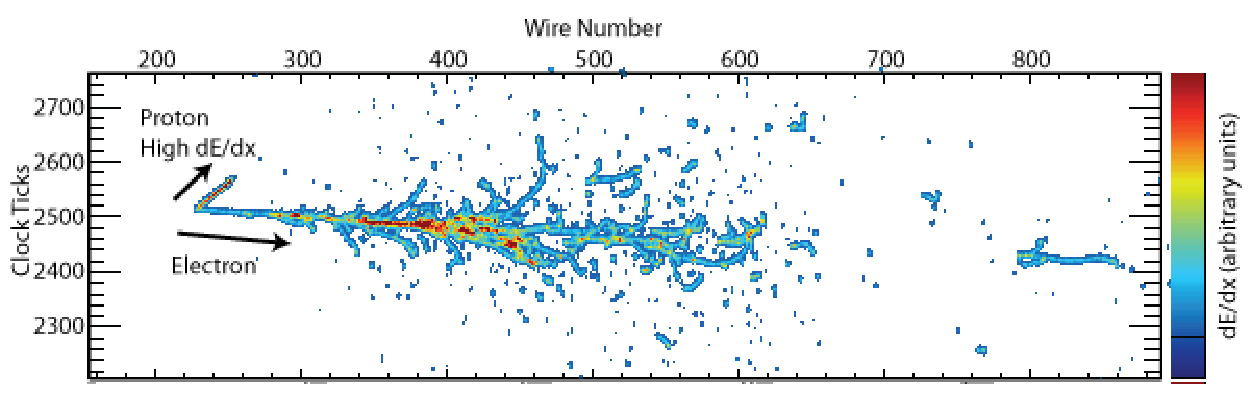
\includegraphics[width=\textwidth]{nueQE_annotated.pdf}
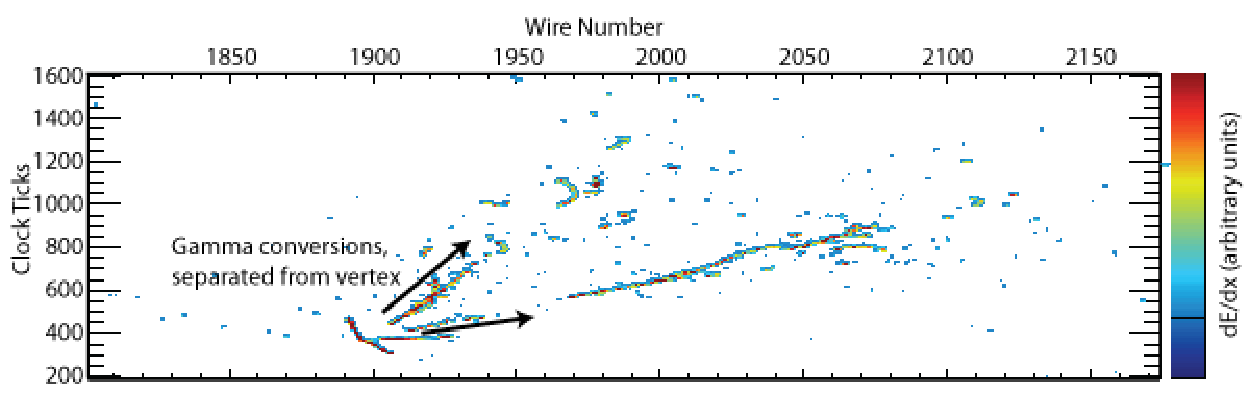
\includegraphics[width=\textwidth]{nc_pi0sep_annotated.pdf}
\end{cdrfigure}

%\subsection{Near Detector Reconstruction}
%\label{sec:detectors-sc-physics-software-reconstruction-nd}

\subsection{Far Detector Reconstruction}
\label{sec:detectors-sc-physics-software-reconstruction-fd}

The reconstruction of particle interactions in Liquid Argon TPC
detectors is an active area of research and development and
there has been considerable progress in recent years. 
In particular, the data from the ICARUS~\cite{Amerio:2004ze,icarus-url,ICARUS-pizero,Antonello:2012hu} 
and ArgoNEUT experiments~\cite{Adamson:2013/02/28tla,argoneut-url,Acciarri:2013met}
have enabled the development of a variety of new reconstruction techniques,
forming the basis for precision measurements of neutrino physics.
With the advancement of both single-phase and dual-phase technologies,
and expansion of the experimental program to include MicroBooNE~\cite{Chen:2007ae,microboone-url},
the 35-ton prototype and the CERN test experiments,
reconstruction tools has continued to grow in both volume and sophistication,
supported by the powerful software frameworks such as LArSoft and Qscan.

A fully automated chain of event reconstruction algorithms
will be developed for the DUNE Far Detector.
The block diagram in figure~\ref{fig:fdrecoblockdiag} illustrates 
the components of this reconstruction chain.
The first stage of reconstruction involves the processing of the
noisy ADC wire signals, and the creation of 2D `hits'. 
These hits provide the input for a series of pattern recognition algorithms,
which form 2D and 3D clusters, representing individual particle tracks and showers.
A set of high-level algorithms are then used to reconstruct the vertex
and 3D trajectory of each particle, identify the type of particle,
and fit the four-momentum.
While each stage of the reconstruction chain has been implemented,
the algorithms are not yet fully optimised and are subject to
continuous improvement.

\begin{cdrfigure}[Far detector reconstruction block diagram]{fdrecoblockdiag}
{Block diagram showing the components of the far detector reconstruction chain}
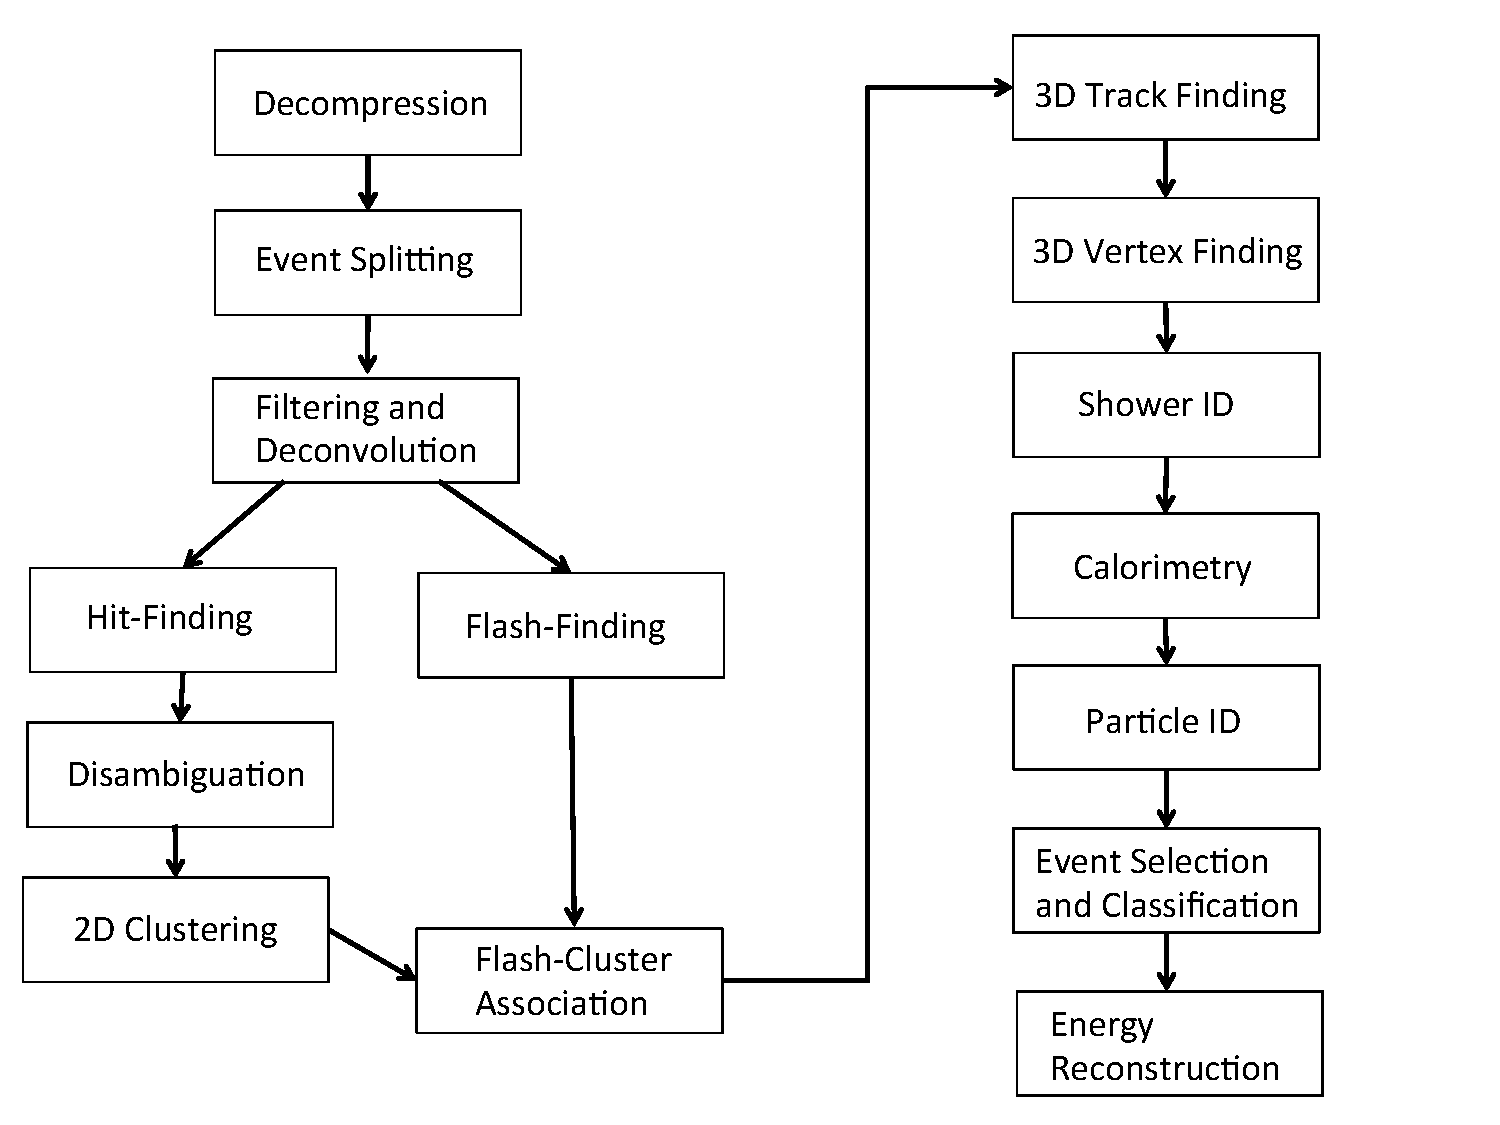
\includegraphics[width=0.8\textwidth]{fdrecoflowchart.pdf}
\end{cdrfigure}


\subsubsection{Signal Processing, Hit Finding, and Disambiguation}

The data are first uncompressed, the noise is reduced by filtering,
and a deconvolution of the detector and electronics response is applied.
The pulse-shape models used to deconvolute the response are currently
based on {\it a priori} predictions, but these will be tuned and
validated using data from the 35-ton prototype and CERN test experiments.
The algorithms are found to perform well in ArgoNeuT analyses~\cite{Anderson:2012vc}.
After deconvolution and pedestal subtraction, pulses are identified in
the waveforms, and parametric fits are applied to extract the size and
shape of each pulse. These pulses are called hits for later processing.
At this stage, the data are still two-dimensional -- each hit provides
a wire location and a measurement of time and total charge,
but no indication of where along a wire the charge was deposited.
Hits may also overlap if they are close together in time, 
even if the charge was deposited on distant segments of the wire.

The wrapping of induction-plane wires in the single-phase Far Detector APA design
introduces an additional discrete ambiguity in the data by connecting multiple wire
segments to each DAQ channel. A ``disambiguation'' algorithm,
described in Section~\ref{annex:reco-disambiguation}, is used to break the
ambiguity and determine which wire segment generated the charge on each hit.
The algorithm forms associations between the collection view and induction views,
identifying ``triplets'' of hits that have intersecting wire segments
and consistent arrival times. In most events, the majority of hits are
associated with a single wire segment, and can be trivially disambiguated.
The remaining hits are then disambiguated by clustering them with trivially disambiguated hits.
The disambiguation procedure constitutes the first pattern recognition stage 
in the single-phase detector.  The performance of the disambiguation algorithm is
discussed in the Annex~\cite{annex:disambiguation}.

\subsubsection{Optical Detector Signal Reconstruction}

Optical detector signals are processed in similar ways to those on the TPC wires.
Noise is filtered out, and hits are identified as pulses above the pedestal.
Hits are grouped together into clusters, called ``flashes'', for subsequent
association with clusters in the TPC.  Each flash has a total integrated charge and a position
estimate.


\subsubsection{TPC Hit Clustering}

After the hit-finding and disambiguation stages have completed, a series of 
pattern recognition algorithms are applied to the 2D hits in order to identify 
the 3D tracks and showers produced by the final-state particles in an event.
The reconstruction of 3D particles is accomplished either by forming 2D clusters
and associating them between views, or by first associating 2D hits between views
and then clustering the resulting 3D hits. 
The clustering of hits in Liquid Argon TPC detectors is a challenging task
due to the variety and complexity of event topologies.
However, several automated 2D and 3D pattern recognition algorithms have been 
implemented using a range of techniques.

One promising suite of reconstruction tools is the 
PANDORA software development kit~\cite{Marshall:2013bda,Marshall:2012hh}
which provides fully-automated pattern recognition for both single-phase 
and dual-phase technologies. 
PANDORA implements a highly modular approach to pattern recognition,
in which events are reconstructed using a large chain of algorithms. 
A series of 2D pattern recognition algorithms are first applied,
which cluster together nearby hits based on event topology.
The resulting 2D clusters are then associated between views
and built into 3D tracks and showers, modifying the 2D clustering 
as needed to improve the 3D consistency of the event. 
Vertex-finding algorithms are also applied,
and neutrino events are reconstructed by associating the 
3D particles to the primary interaction vertex.
The PANDORA algorithms have been developed using accelerator neutrinos 
in the energy range 100\,MeV\,$-$\,25\,GeV.
Figure~\ref{fig:pandoraefficiency} shows the efficiency for reconstructing
the leading final-state lepton as a function of its momentum
for 5\,GeV $\nu_{e}$ and $\nu_{\mu}$ charged-current interactions
simulated in the MicroBooNE detector.
In both samples, the reconstruction efficiency increases rapidly with momentum,
rising above 90\% at 500\,MeV and reaching approximately 100\% at 2\,GeV.

\begin{cdrfigure}[PANDORA reconstruction efficiency]{pandoraefficiency}
{Reconstruction efficiency of Pandora pattern recognition algorithms
 for the leading final-state lepton in 5\,GeV $\nu_{\mu}$ CC (left) and
 $\nu_{e}$ CC (right) neutrino interactions, plotted as a function of
 the lepton momentum. The reconstruction performance is evaluated
 using the MicroBooNE detector geometry. }
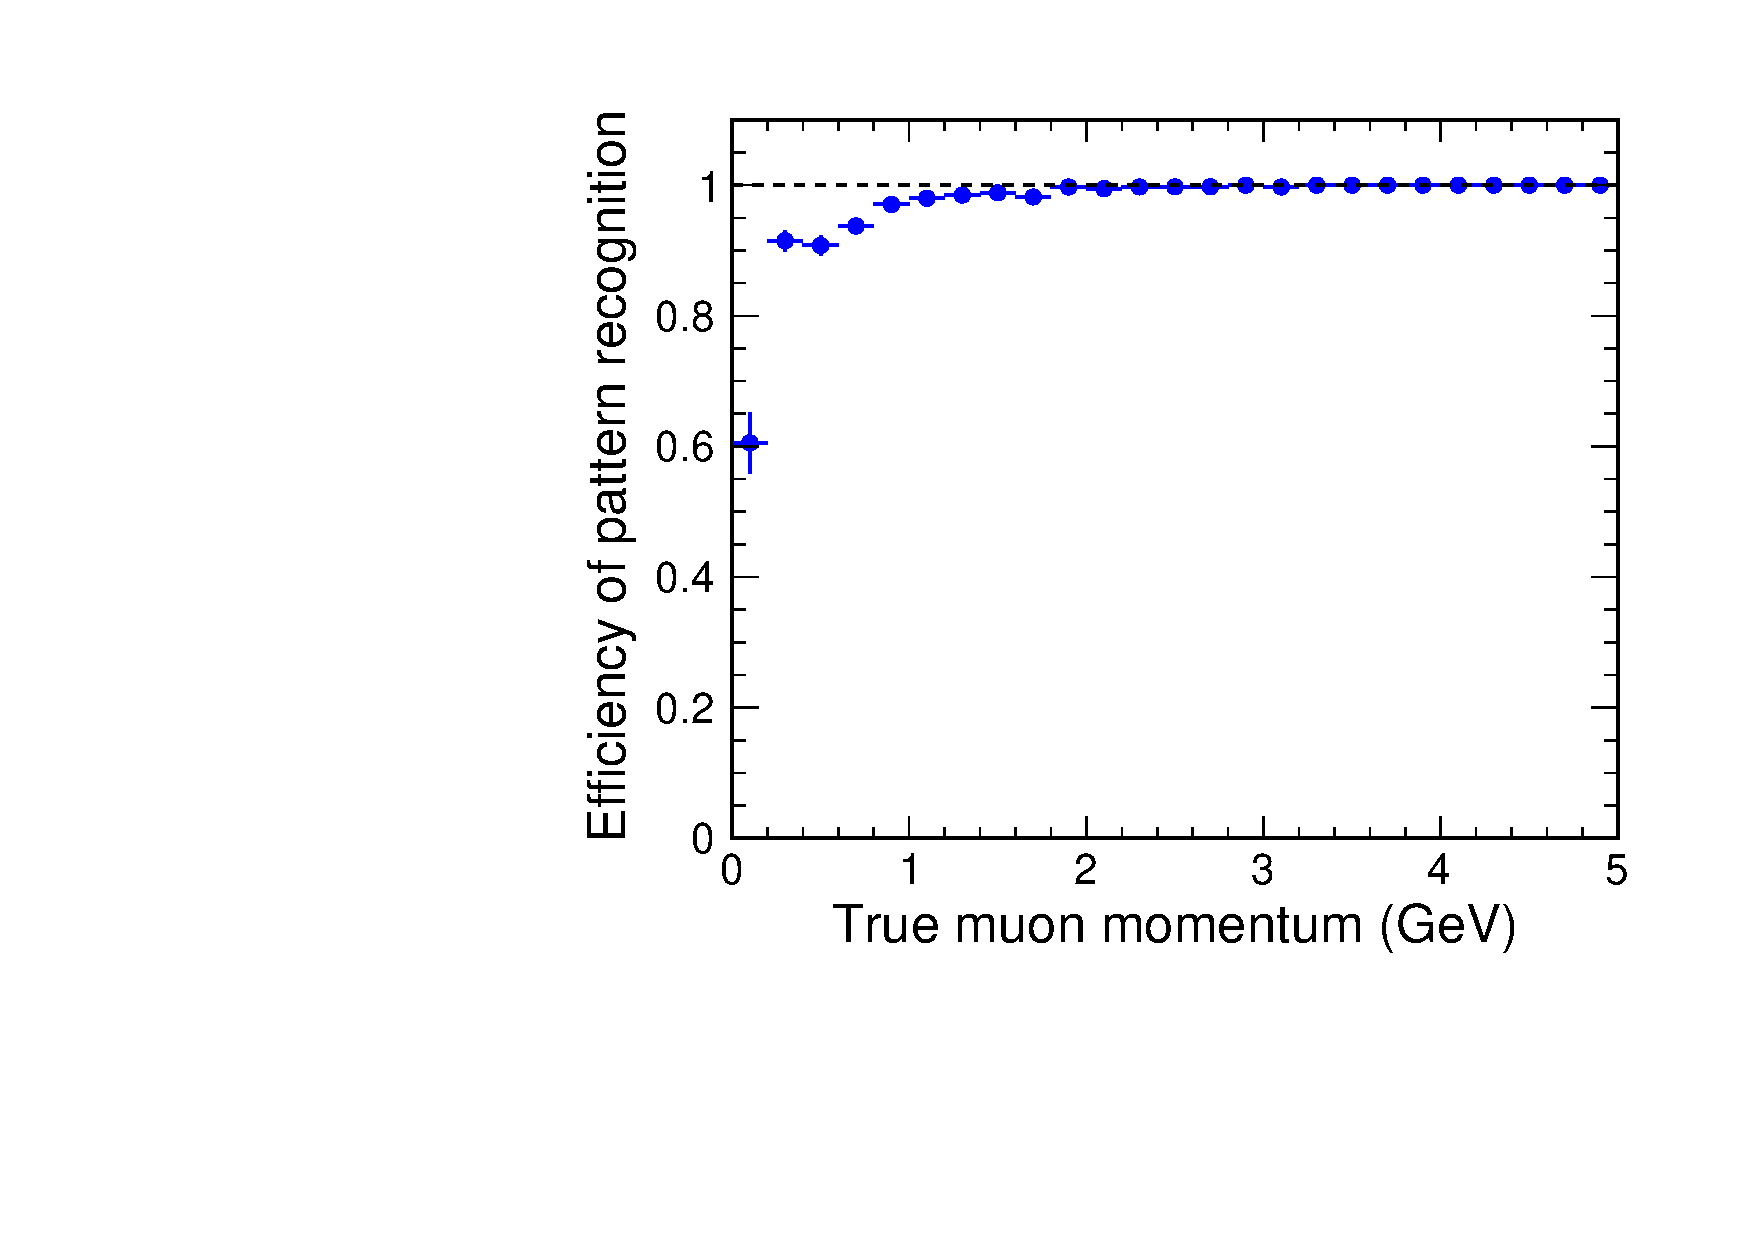
\includegraphics[width=0.49\textwidth]{pandora_uboone_efficiency_5GeV_numucc.pdf}
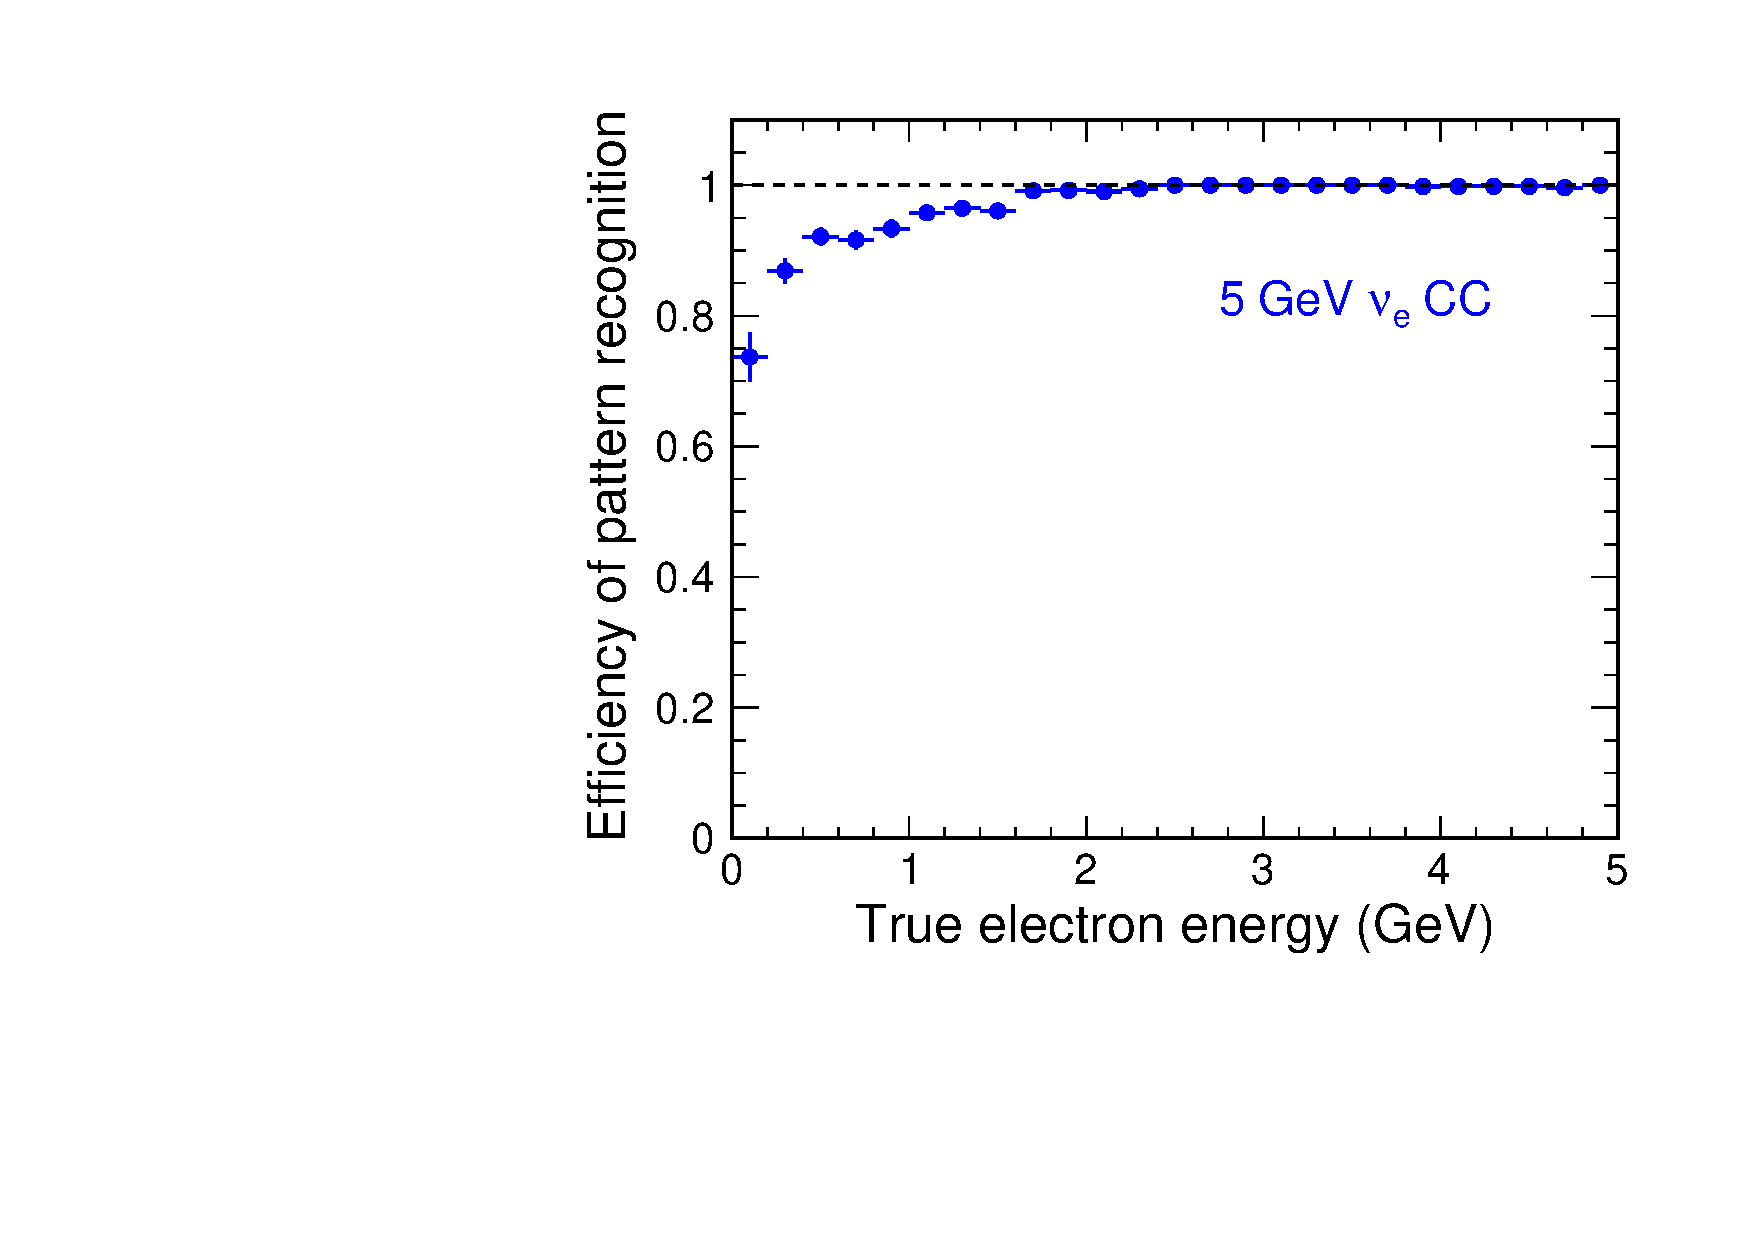
\includegraphics[width=0.49\textwidth]{pandora_uboone_efficiency_5GeV_nuecc.pdf}
\end{cdrfigure}


\subsubsection{Track Fitting and Shower Measurement}

The reconstruction of LArTPC events benefits greatly from multiple algorithms
performing similar reconstruction tasks, as ideas from one development line
can be applied to another, and the best algorithm chosen for a particular 
purpose.

Tracks may be reconstructed also with a Kalman Filter algorithm~\cite{kalman}.
In this algorithm, hits are combined from multiple views for form three-dimensional
space points.  Three-dimensional track reconstruction can proceed from space points
or directly from hits.

\fixme{Talk about local principal curves here, and show vertex resolution plots}

%Figure~\ref{fig:vertexresolution} Shows resolution [Citation: Eur. Phys. J. C (2014), 74 - 2832]
%
%\begin{cdrfigure}[Vertex resolution from local principal curves]{vertexresolution}
%{CAPTION GOES HERE}
%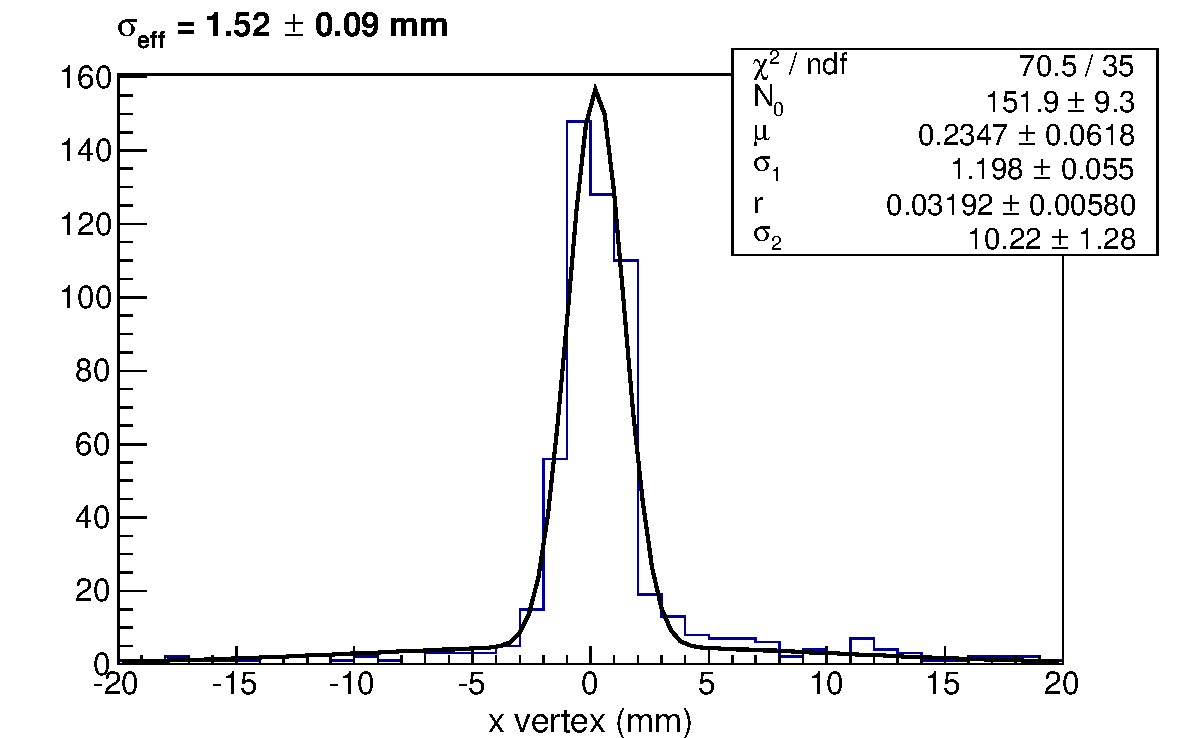
\includegraphics[width=0.33\textwidth]{barker_vertex_nueccqe_x.pdf}
%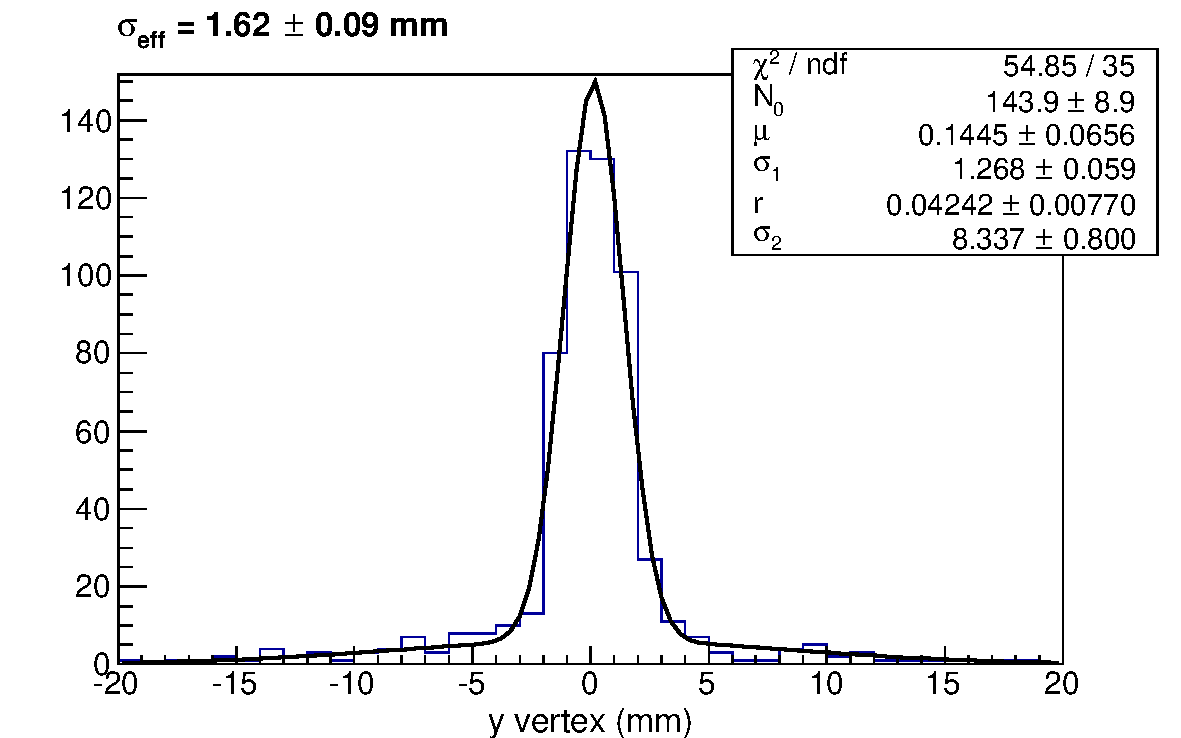
\includegraphics[width=0.33\textwidth]{barker_vertex_nueccqe_y.pdf}
%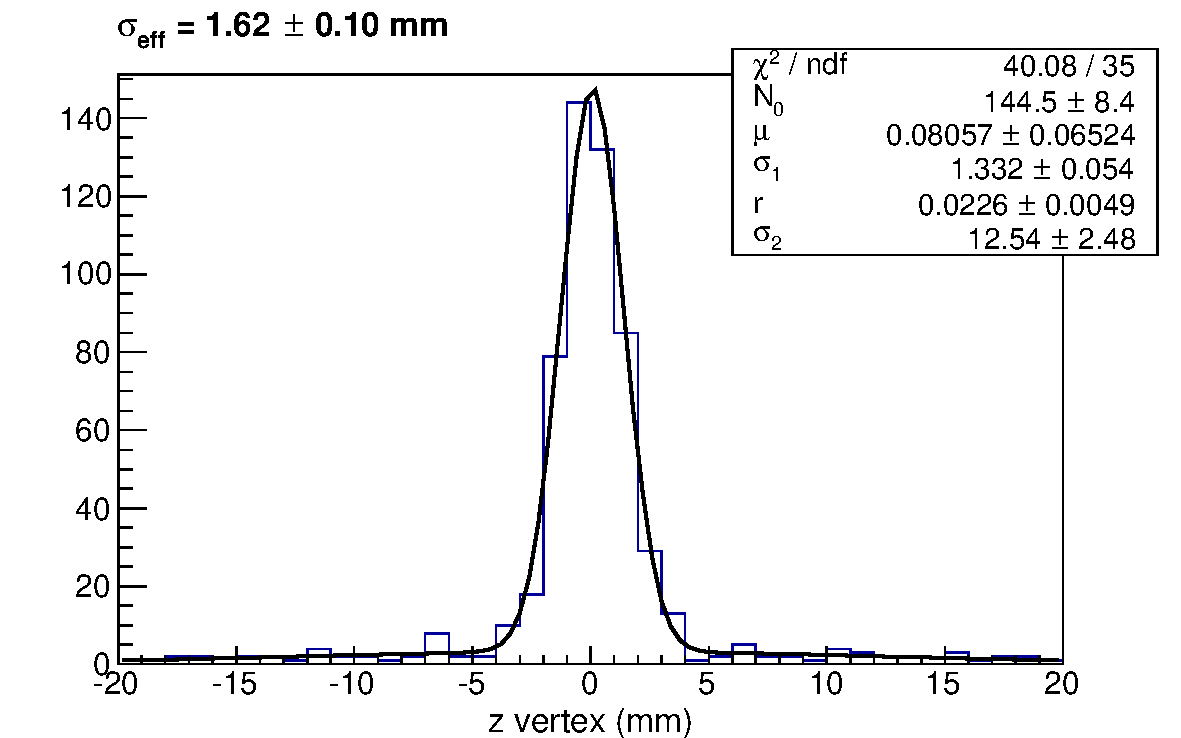
\includegraphics[width=0.33\textwidth]{barker_vertex_nueccqe_z.pdf}
%\end{cdrfigure}

The electromagnetic shower algorithms have two
steps. The first is a post-clustering stage which examines the
existing clusters in terms of their 2D parameters to determine whether
the clusters are shower-like or track-like. 
The selected shower-like clusters are examined to assign starting points,
directions and angles in the wire-time plane. The second step is 
3D shower reconstruction, which
matches the 2D clusters between views in order to obtain 3D shower axes and start points.
These 3D parameters allow the calculation of the shower energies and charge
depositions at the starts of the showers, which are used in particle
identification. 

\fixme{Can we say something about current status or performance of the shower reconstruction?}

\subsubsection{Calorimetry and Particle ID}

The measurement of the ionization density $dE/dx$ is important
for particle identification and energy measurement.
The algorithm for reconstructing the ionization
energy in LArSoft is optimized for line-like tracks and is being
extended to showers.  The measured charge on each hit is obtained from
fits to the pulse shapes in ADC counts vs. time, and calibrated to units
of fC.  The charge loss due to the finite electron lifetime is corrected for
using the time of the event.  Geometrical effects from the track angle are
included as the amount of path length corresponding to each hit depends on the
track and wire angles.  The effects of recombination, known as ``charge quenching''
are corrected using a modified Box model~\cite{box} or Birks' Law`\cite{birks}.

\fixme{Borrow performance plot from LBNE Science Opportunities document?}

The identity of charged particles which range out in the LArTPC active
volume may be ascertained by comparing the ionization density $dE/dx$ as a function
of residual range, the distance from a point along the track to the end of the
track, with predictions for different particle species.  Various techniques,
from $\chi^2$ comparisons to neural networks to the PIDA variable described
in Section~\ref{annex:reco-pid}~\cite{Acciarri:2013met}.
 
\fixme{LBNO}
In Qscan, a multivariate analysis was used to separate particle types based on the spatial characteristics of their clusters.
Several quantities are calculated to 
characterize the cluster: the lateral spread, the mean charge-weighted inverse distance of hits to the primary cluster axis
(this is expected to distinguish effectively between showers and tracks), the $dE/dx$.
These variables are then fed into Boosted Decision Trees analyses, 
each calculating the signal and background likelihoods for a particular particle hypothesis

The overall performance of the reconstruction chain (from clustering to PID) has been estimated with a simple binned lepton flavour analysis, 
to understand its ability to distinguish $\nu_{e}$ and $\nu_{\mu}$ events.
If a single lepton flavour is identified in the event, then the event is considered as a signal event of the observed lepton flavour. 
If neither or both lepton flavours are identified, the event is discarded.
Numbers of events correctly reconstructed is above 90$\%$ for $\nu_{\mu}$-CCQE events.
assuming that all hits not associated with the lepton cluster are due to hadronic activity.

\fixme{Current results?}


